\documentclass[11pt]{article}
\usepackage[margin=1in]{geometry}
\usepackage{tikz}
\usetikzlibrary{positioning,arrows,shapes,backgrounds}

%===========================================================================================
\pgfdeclarelayer{background layer}
\pgfsetlayers{background layer,main}

\tikzset{
	block base/.style={draw, rectangle, rounded corners},
}

%===========================================================================================
\begin{document}

asfsf asdfsdf asdfsdfflkfasdf adf kadfjadf asdf asdfjkdasdf fasdf.

\noindent
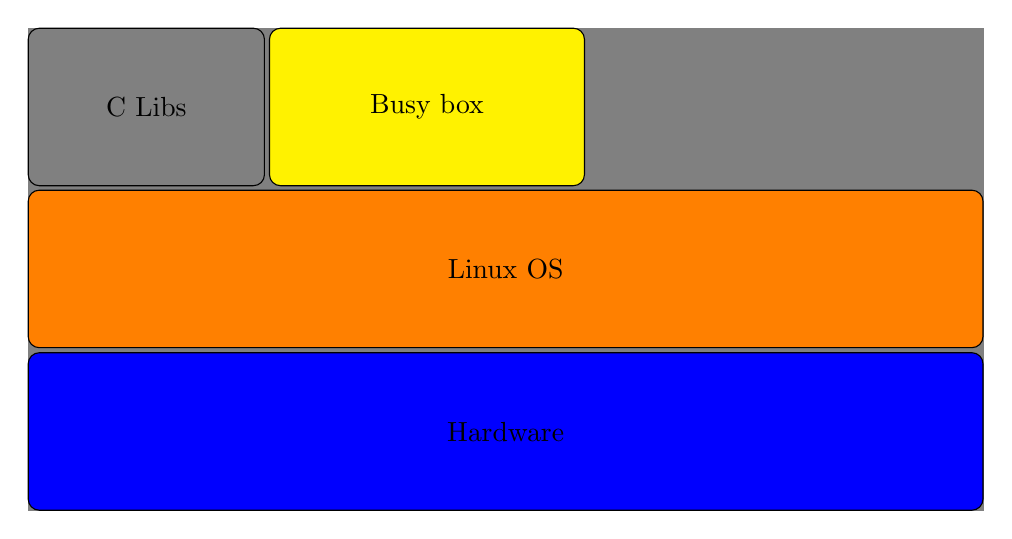
\begin{tikzpicture}
	% On main layer
	\node [block base,minimum width=\textwidth,minimum height=20mm,fill=orange] (os) {Linux OS};
	\node [block base,minimum width=\textwidth,minimum height=20mm,fill=blue,below=0.5mm of os] {Hardware};
	\node [block base,minimum width=30mm,minimum height=20mm,fill=gray,above=10.5mm of os.north west,anchor=west] (clib) {C Libs};
	\node [block base,minimum width=40mm,minimum height=20mm,fill=yellow,right=0.5mm of clib.east] (busybox) {Busy box};

	%\draw[step=1cm,gray,very thin] (0,0) grid (10,10);
	%\draw[step=1cm,gray,very thin] (-10,-10) grid (0,0);
	% On block 1 layer
	\begin{pgfonlayer}{background layer}
	\fill [gray] (current bounding box.south west) rectangle (current bounding box.north east);
	\end{pgfonlayer}

\end{tikzpicture}

\end{document}
%===========================================================================================
